\documentclass{article}

% if you need to pass options to natbib, use, e.g.:
% \PassOptionsToPackage{numbers, compress}{natbib}
% before loading nips_2018

% ready for submission
\usepackage[preprint]{nips_2018}

% to compile a preprint version, e.g., for submission to arXiv, add
% add the [preprint] option:
% \usepackage[preprint]{nips_2018}

% to compile a camera-ready version, add the [final] option, e.g.:
% \usepackage[final]{nips_2018}

% to avoid loading the natbib package, add option nonatbib:
% \usepackage[nonatbib]{nips_2018}

\usepackage[utf8]{inputenc} % allow utf-8 input
\usepackage[T1]{fontenc}    % use 8-bit T1 fonts
\usepackage[draft]{hyperref}       % hyperlinks
\usepackage{url}            % simple URL typesetting
\usepackage{booktabs}       % professional-quality tables
\usepackage{amsfonts}       % blackboard math symbols
\usepackage{nicefrac}       % compact symbols for 1/2, etc.
\usepackage{microtype}      % microtypography
\usepackage{amsmath}
\usepackage{graphicx}
\usepackage{algorithm, algpseudocode}



\title{Final Project}

\author{
  Kevin Shi\\
  Columbia University\\
  \And
  Harvey Wu \\
  Columbia University \\
}

\begin{document}
% \nipsfinalcopy is no longer used

\maketitle

\begin{abstract}
The aim of this project is to investigate the effectiveness of various meta-learning approaches on the OpenAI Retro Contest, a recently launched benchmark based on the video game series \emph{Sonic the Hedgehog} \citep{retro}. We re-implement two baseline algorithms (PPO and Joint PPO) from the Retro Contest technical report and experiment with approaches from hierarchical and memory-based reinforcement learning.
\end{abstract}

\section{Introduction}
Games are intimately tied to the field of reinforcement learning. The rise of deep RL, foreshadowed by TD-Gammon \citep{tesauro}, has lead to systems that can tackle games of huge state spaces such as Go\citep{silver}. The Arcade Learning Environment (ALE), including a varied collection of Atari games, has been an important benchmark for all flavors of RL algorithms \citep{ale}. In this work, we explore a meta-learning task: whether an agent can learn to play new games through leveraging the knowledge gained from previously solved games. Our benchmark for evaluation is the newly released OpenAI Retro Contest, a selection of various levels from three releases of \emph{Sonic the Hedgehog} \citep{retro} divided into training and evaluation sets. The problem that the Retro Contest aims to tackle has important implications for reinforcement learning. Although RL agents can achieve superhuman performance on many Atari games, they are extremely sample inefficient compared to humans and require large amounts of computing power to learn \citep{lake}. Additionally, RL agents find it difficult to generalize between similar games, even if the goals and underlying physics of said games are mostly identical. This is evidenced by the poor performance of the baseline algorithms in the Retro Contest technical report: humans perform [...] times better than the highest performing algorithm, [...]. An agent that consistently achieves robust performance on the Retro Contest will possibly bring insight to similar problems in RL beyond the realm of games, such as


\section{Related Work}

Meta-learning has often been approached in the context of "few-shot learning", or learning with little sample data. Datasets such as Omniglot \citep{lake} and miniImagenet \citep{} \citep{} view few-shot learning from the lens of image classification. Modified deep learning architectures \citep{} \citep{} \citep{} have been introduced to tackle these two datasets, seeing mixed success on miniImagenet but basically "solving" Omniglot (the cited models all report accuracies of >95\%). However, such architectures do not have natural extensions to a reinforcement learning setting. MAML \citep{maml} was the first architecture to generalize to RL, reporting results on [...]. 

\section{Approaches}
\subsection{Model-free}
Policy gradient algorithms are model-free in the sense that they implicitly integrate out the state transition model when performing Monte Carlo estimation of the reward function. This has the advantage of being able to represent more complicated policies than the greedy algorithm with a DQN, but as a tradeoff more of the work is being offloaded to the deep learning black box. Because of this fact, it is more difficult to understand transfer learning of the learned policy network between different tasks. 

Proximal Policy Optimization (PPO) is the main policy gradient algorithm we use. We consider here both vanilla PPO, where an agent is individually trained on all training levels, and "joint" PPO, where multiple instances are trained in parallel with shared gradient information. \citep{retro} report a significant performance boost when PPO is "joint-ed", but no such boost for their Q-learning based method.

In each training epoch, we play at least 5 minutes / 4500 time steps worth of gameplay using the current policy network. Each trajectory is terminated if the agent spends more than 600 time steps without acquiring any reward. If the agent does not have 4500 time steps of training data, a new trajectory is started. 

\subsection{Model-based}

In model-based RL, we try to explicitly understand the state transition dynamics of the environment. This lends itself more naturally to transfer learning between different Sonic levels, because the basic 2D physics of the game are universally applicable beyond the specific layout of a particular level. Another benefit of learning an explicit state transition model is enabling more effective exploration, because the agent only needs to explore sequences of actions that actually change the agent's state. 

One recent paper discussing learning the dynamics of the environment is \citep{Ha2018WorldModels}, where the authors train a full generative model to sample possible subsequent states. It remains to incorporate the training procedure of such a model with reinforcement learning methods. Because Sonic has simple 2D physics, the state transition model may be able to be captured by a much simpler transition network. 

\section{Experiments}

We show the performance of the model-free PPO algorithm on two Sonic test levels. The rewards on the y-axis are scaled by 0.01, so the maximum reward for beating a level is between 90 and 100 depending on completion time.

Figure (\ref{fig:ghza1}) shows that the agent is able to learn to consistently navigate a little over half of the level after a significant amount of training time, and the reward of the agent's policy continues to improve with training time. The Green Hill Zone Act 1 level is simple in terms of navigation, so the agent only needs to learn to avoid dying to enemies and obstacles along the way.

However for the more complicated Labyrinth Zone Act 1, Figure (\ref{fig:lza1}) shows that the PPO agent makes almost no progress beyond the first few training epochs. This level has initial enemies which are almost entirely avoidable just by holding down R and jumping. However the agent gets stuck at a region of the level which requires Sonic to jump up and backwards out of the water, and then wait for a moving platform to come over. Unfortunately it is far beyond the capability of PPO to explore such a possible trajectory. 

\begin{figure}
	\begin{minipage}{0.5\textwidth}
		\begin{center}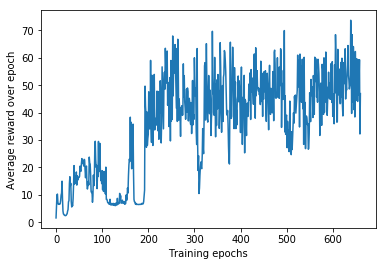
\includegraphics[width=0.95\textwidth]{greenhillzone.png}\end{center}
		\caption{Green Hill Zone, Act 1}
		\label{fig:ghza1}
	\end{minipage}
	\begin{minipage}{0.5\textwidth}
		\begin{center}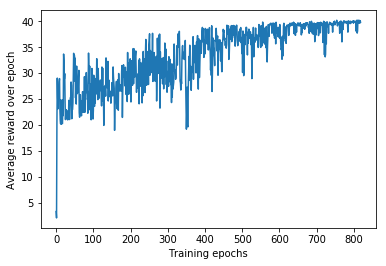
\includegraphics[width=0.95\textwidth]{labyrinthzone.png}\end{center}
		\caption{Labyrinth Zone, Act 1}
		\label{fig:lza1}
	\end{minipage}
\end{figure}


\section{Discussion and Conclusion}


\medskip

\small

\bibliographystyle{unsrtnat}
\bibliography{biblio}

\end{document}
